%%%%%%%%%%%%%%%%%%%%%%%%%%%%%%%%%%%%%%%%%%%%%%%%%
%%%
%%% Auteur : Stéphane Péchard - stephane.pechard@univ-nantes.fr
%%% Fichier : 5-eval.tex - chapitre 5 :  Évaluation de critères sur une base de séquences haute définition (15 pages)
%%% Version : 0.1
%%% Date : 2008/02/12
%%%
%%%%%%%%%%%%%%%%%%%%%%%%%%%%%%%%%%%%%%%%%%%%%%%%%
\chapter{Performances de critères objectifs de qualité visuelle en télévision haute définition} \label{chap:evalCrit}
\opt{final}{\lettrine[lines=4]{U}{n critère objectif de qualité visuelle}}\opt{nofinal}{Un critère objectif de qualité visuelle} doit produire une grandeur reflétant autant que possible le jugement humain. Mesurer la fidélité du critère objectif à ce jugement humain revient à évaluer le critère correspondant. La question de l'évaluation des critères est cruciale. En effet, elle permet d'une part de connaitre les performances d'un critère vis-à-vis du jugement subjectif, et d'autre part de disposer d'indicateurs permettant la comparaison des critères objectifs entre eux. Pourtant, il est rare que les auteurs de critères objectifs fournissent un ensemble complet de tels indicateurs de performance. Nous cherchons donc ici à nous doter de mesures de performance mais également de moyens de distinguer si les mesures obtenues par deux critères sont significativement différentes ou pas.

Une fois ces outils définis, nous proposons de les mettre en application. Nous avons constaté qu'aucun critère de qualité vidéo n'était spécialisé dans l'évaluation de la qualité de la TVHD. Bien que nous ayons montré des différences sensibles entre la TVHD et la TVSD, peut-être que des critères existants peuvent prédire de manière efficace la qualité visuelle de la TVHD. Nous devons donc savoir comment des critères performants en TVSD s'adaptent à ce contexte différent. Ainsi, nous avons évalué deux critères de qualité vidéo avec référence complète sur une base de séquences de télévision haute définition. Pour cela, nous utiliserons la base présentée à l'annexe~\ref{annex:base}. Le premier critère est une adaptation à la vidéo du critère pour images fixes SSIM~\cite{wang-vqasdm}. Celui-ci est bien connu des universitaires de la communauté de la qualité d'image. Le second est le VQM de Wolf et Pinson~\cite{wolf-vqmtech}, plus connu des instances de normalisation. Il est l'un des meilleurs critères de la seconde campagne d'évaluation de VQEG~\cite{vqeg-frtv2}. Ce type de banc d'essai est intéressant dans la mesure où les auteurs des critères sont souvent les seuls à évaluer leurs propres travaux. Utiliser un critère connu dans différentes conditions, et notamment sur une base de séquences différente, fournit à la communauté scientifique de précieux enseignements sur ses capacités.

L'objectif de ce chapitre est donc double. Dans un premier temps, nous présenterons divers outils utiles au calcul des performances d'un critère. Nous y détaillerons également des méthodes de différenciation de certaines mesures de performance. Dans un second temps, nous utiliserons ces mesures de performance pour évaluer les deux critères de qualité vidéo testés.


\section{Validation des critères de qualité}
À partir de séquences d'une base de vidéos à tester comme celle de l'annexe~\ref{annex:base}, un critère objectif de qualité génère autant de notes objectives de qualité que de séquences. Avant de mesurer les performances du critère, ces notes sont souvent transformées en prédiction des mesures subjectives correspondantes par une fonction d'ajustement \emph{(mapping)}. Ceci est illustré sur la figure~\ref{fig:definMOS} où MS est un ensemble de mesures subjectives, NO un ensemble de notes objectives et MSP l'ensemble des prédictions. Typiquement, les mesures subjectives sont des MOS ou des DMOS. Les prédictions correspondantes sont respectivement notées MOSP et DMOSP. Les premières sont utilisées pour des mesures de qualité, alors que les secondes sont plutôt associées aux mesures de fidélité. Typiquement, les performances des critères avec référence complète sont calculées entre les NO et les DMOS.

\begin{figure}[htbp]
\centering
\begin{tikzpicture}[node distance=3cm]
\node (mos) {MS};
\node[action, below of=mos, text width=2cm, node distance=1.7cm] (func) {fonction d'ajustement};
\node[below of=func, node distance=1.7cm] (no) {NO};
\node[right of=func] (mosp) {MSP};
\node[action, right of=mosp, text width=2cm] (perf) {mesures de performance};
\node[right of=perf] (mesures) {cc, reqm, or, etc.};

\draw[fleche] (mos) -- (func);
\draw[fleche] (no) -- (func);
\draw[fleche] (func) -- (mosp);
\draw[fleche] (mosp) -- (perf);
\draw[fleche] (perf) -- (mesures);
\draw[fleche] (mos) -| (perf);

\end{tikzpicture}
\caption{Obtention des mesures de performance à partir des mesures subjectives MS et des notes objectives NO d'un ensemble de séquence.}
\label{fig:definMOS}
\end{figure}

La fonction d'ajustement a plusieurs buts. Le premier est d'adapter la dynamique des notes objectives à celle des mesures subjectives afin de pouvoir les comparer. Le second est de prendre en compte des phénomènes de saturation qui peuvent apparaitre au niveau des limites de l'échelle. Ces phénomènes dépendent de plusieurs choses comme la répartition des dégradations de l'ensemble de séquences ou la présence ou non d'une ancre basse dans la méthodologie d'évaluation subjective de la qualité. L'usage de telles fonctions peut cependant paraitre discutable. En effet, cela permet de compenser un phénomène courant du jugement humain. Ce phénomène est dû au fait que les ancres de haute et basse qualité tirent le jugement vers les extrémités car il est plus difficile de différencier les très basses ou les très bonnes qualités. Pourtant, la question qui se pose est de savoir si ce phénomène ne devrait pas être pris en compte par les critères objectifs, puisqu'il correspond à une réalité subjective. Pourtant, l'usage actuel veut qu'une telle fonction n'est pas incluse dans le critère, c'est pourquoi nous procéderons de même.

Les performances d'un critère sont ensuite mesurées entre les MS et les MSP correspondants. Les aspects à caractériser sont la précision, la monotonie et la cohérence de la relation. Afin de les évaluer, VQEG préconise l'usage de plusieurs mesures de performance~\cite{vqeg-MMtestplan}. Il est rare de voir l'usage de plus d'une ou deux mesures dans la littérature universitaire. Par exemple, certains auteurs ne fournissent que le coefficient de corrélation~\cite{eskicioglu-icassp2000,wang-icip2002,ebrahimi-spie2004,crete-phd}, auquel Oelbaum~\cite{oelbaum-pcs2007} ajoute l'\emph{outlier ratio}. Watson n'utilise quant à lui que la racine carrée de l'erreur quadratique moyenne~\cite{watson-dvq} pour évaluer son critère DVQ. Quelques auteurs seulement~\cite{chen-icassp2006,chandler-vsnr} en fournissent plus. Or, nous pensons que la complexité de la relation entre des mesures subjectives et des notes objectives ne peut se caractériser par une ou deux valeurs. Le coefficient de corrélation seul ne suffit pas à décrire les performances d'un critère de manière pertinente. De plus, il nous semble important de pouvoir comparer des performances évaluées sur des ensembles de vidéos de taille différente. En effet, la précision de la mesure de performance dépend du nombre de séquences utilisées. Pour pouvoir comparer des critères de précisions différentes, il existe des outils de calcul de la signifiance des différences entre mesures de performance. Encore une fois, ces outils sont peu utilisés dans le domaine universitaire.

Cette section présente donc plusieurs outils d'analyse des données issues des critères objectifs de qualité. Dans un premier temps, nous détaillerons la manière de générer des prédictions de mesures subjectives par une fonction d'ajustement. Puis, des mesures de performances et des outils pour les différencier seront données et discutées.


\subsection{Fonction d'ajustement}
Une telle fonction doit remplir deux conditions~\cite{brill-spic}. La première est qu'elle doit être définie pour les valeurs de mesures subjectives et de notes objectives traitées. La seconde est qu'elle doit être monotone sur le domaine de définition afin de conserver l'ordre des valeurs. Il existe évidemment un grand nombre de fonctions remplissant ces conditions, mais pour diverses raisons, certaines sont plus particulièrement préconisées ou adoptées. Par exemple, VQEG~\cite{vqeg-MMtestplan} a déterminé de manière empirique une fonction d'ajustement polynomiale :
\begin{equation}
\text{MSP}_1 = a x^3 + b x^2 + c x + d
\end{equation}
%
avec $a$, $b$, $c$ et $d$ quatre paramètres d'adaptation. La variable $x$ représente la note objective d'origine. L'ajustement consiste à minimiser la racine carrée de l'erreur quadratique moyenne entre les DMOS et les DMOSp en ajustant les quatre paramètres.

Une seconde fonction très utilisée est la fonction psychométrique suivante :
\begin{equation}
\text{MSP}_2 = \frac{a}{1+e^{-b(x - c)}} \label{eq:funcPsycho}
\end{equation}
%
avec $a$, $b$ et $c$ les trois paramètres à optimiser. $a$ correspond à la dynamique totale de la fonction, $b$ est lié à la pente et $c$ au décalage par rapport à l'origine. La figure~\ref{fig:foncAjust} présente un exemple de ces deux fonctions d'ajustement : figure~\ref{fig:foncAjustCubic} pour la fonction polynomiale cubique (avec $a$ = -1, $b$ = 3 et $c$ = $d$ = 1 sur un domaine où elle reste monotone) et figure~\ref{fig:foncAjustPsycho} pour la fonction psychométrique (avec $a$ = 1 et $b$ = $c$ = 2). Nous constatons sur ces figures la prise en compte des effets de saturation que nous avons décrits.

\shorthandoff{:} % debug pgf
\begin{figure}[htbp]
	\centering
	\subfloat[\label{fig:foncAjustCubic}Fonction d'ajustement polynomiale cubique avec $a$ = -1, $b$ = 3 et $c$ = $d$ = 1.]{%
	\begin{tikzpicture}[domain=0:2.2,xscale=2.1,yscale=0.8]
		\draw[->] (-0.042,0) -- (2.5,0) node[right] {$x$};
		\draw[->] (0,-0.175) -- (0,7.7) node[above] {$\mathit{DMOSp}_1$};
		\node[below] at(0,-0.175) {0};
		\draw (1,0) -- (1,-0.175) node[below] {1};
		\draw (2,0) -- (2,-0.175) node[below] {2};
		\draw (0,1) -- (-0.042,1) node[left] {1};
		\draw (0,7) -- (-0.042,7) node[left] {7};
		\draw plot function{-x*x*x + 3*x*x + x +1};
	\end{tikzpicture}}\hfill
	\subfloat[\label{fig:foncAjustPsycho}Fonction d'ajustement psychométrique avec $a$ = 1 et $b$ = $c$ = 2.]{%
	\begin{tikzpicture}[domain=-1:5,yscale=5.6]
		\draw[->] (-1,0) -- (5.5,0) node[right] {$x$};
		\draw[->] (0,-0.02) -- (0,1.1) node[above] {$\mathit{DMOSp}_2$};
		\node[below] at(0,-0.02) {0};
		\draw (2,0) -- (2,-0.02);
		\node[below] at(2,-0.005) {$b$};
		\draw (0,1) -- (-0.1,1) node[left] {1};
		\draw (0,0.5) -- (-0.1,0.5) node[left] {0.5};
		\draw plot function{1/(1+exp(-2*(x-2)))};
	\end{tikzpicture}}
	\caption{Forme de deux fonctions d'ajustement.}
	\label{fig:foncAjust}
\end{figure}
\shorthandon{:}


\subsection{Mesures de performance}
Un critère objectif de qualité qualifié d'efficace doit prédire les mesures subjectives de manière précise, monotone et cohérente. Afin d'évaluer ces trois aspects, VQEG a défini plusieurs mesures que nous allons décrire. De plus, nous introduirons des mesures plus originales encore peu utilisées.


\subsubsection{Mesures de précision}
Les premières mesures de performances rendent compte de la précision de la prédiction. Plus elles sont faibles, plus le critère est précis. Il s'agit de la racine carrée de l'erreur quadratique moyenne :
\begin{equation}
\text{reqm} = \sqrt{\dfrac{1}{N_n - N_p} \sum\limits_{i=1}^N \left(\MS(i) - \MSP(i) \right)^2}
\end{equation}
%
et de la racine carrée de l'erreur quadratique moyenne pondérée par l'intervalle de confiance :
\begin{equation}
\text{reqmp} = \sqrt{\dfrac{1}{N_n - N_p} \sum\limits_{i=1}^N \left( \dfrac{\MS(i) - \MSP(i)}{\IC(i) + \text{0,025}} \right)^2}
\end{equation}
%
avec $\IC(i)$ l'intervalle de confiance à 95\% de la mesure subjective $\MS(i)$, $i$ l'index sur les $N_n$ notes considérées et $N_p$ le nombre de paramètres de la fonction d'ajustement utilisée. Ainsi, avec la fonction psychométrique présentée précédemment, $N_p$ = 3. La valeur constante de 0,025 est ajoutée afin de stabiliser la mesure en cas d'intervalle de confiance de mesure très faible.

Brill~\cite{brill-spic} considère que les mesures classiques de précision ne prennent pas suffisamment en compte la variabilité inter-observateurs. Pour y remédier, il propose une mesure plus évoluée, basée sur le calcul d'une puissance résiduelle. Celle-ci est définie comme la différence $\Delta \mathit{OVQM}$ au-dessus de laquelle les notes subjectives correspondantes aux deux notes objectives de la différence sont statistiquement différentes. Pour calculer cette puissance, les auteurs utilisent le test \emph{t} de Student~\cite{gosset-biometrika} sur les notes objectives. Il est réalisé par paires de séquences dégradées, définissant ainsi un ensemble de différences entre notes objectives. Ce test permet de déterminer si deux signaux sont distincts ou non par l’étude de leur moyenne et de leur écart-type. Il fournit également la probabilité $p$ pour qu'entre deux séquences dégradées, celle obtenant la plus grande note objective soit celle de plus grande mesure subjective. La figure~\ref{fig:brill1} présente l'évolution de cette probabilité en fonction de $\Delta \mathit{OVQM}$ pour le PSNR et le JND de Lubin~\cite{lubin-jnd} dont les résultats sont issus de VQEG Phase 1~\cite{vqeg-frtv1}. Cette méthode originale confirme les résultats obtenus par VQEG, à savoir une faible distinction entre les deux méthodes. En revanche, elle nécessite des calculs plus complexes que les indicateurs classiques, ce qui peut restreindre son utilisation.

\begin{figure}[htbp]
	\centering
	\subfloat[\label{fig:brill1}Probabilité $p$ en fonction de $\Delta \mathit{OVQM}$ pour le PSNR et la version de JND de Lubin~\cite{lubin-jnd}.]{
	\begin{tikzpicture}[text centered]% \begin{tikzpicture}
\node at (0,0) {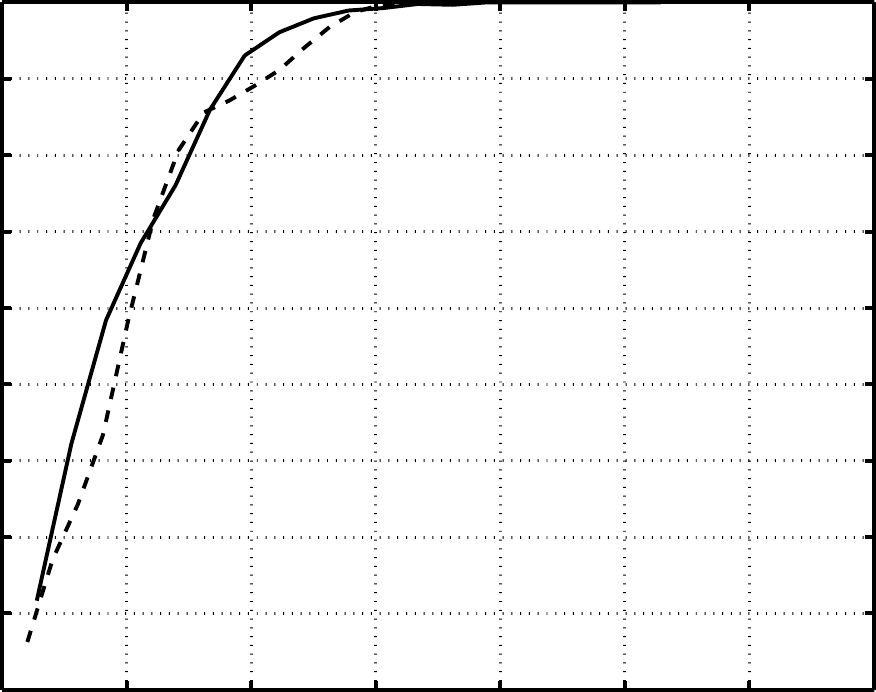
\includegraphics[width=6cm]{img/chap5/brill_refait}};

\draw[legende] (0,0) rectangle (2,-1.3);

\draw (0.1,-0.4) node[anchor=west] {JND};
\draw (0.1,-0.9) node[anchor=west] {PSNR};
\draw[thick] (1.3,-0.36) -- (1.9,-0.36);
\draw[thick, dashed] (1.3,-0.86) -- (1.9,-0.86);

\node[below=0.3cm] at (-3.8,0.5) {$p$};
\node[anchor=east] at (-2.9,-2.35) {0,55};
\node[anchor=east] at (-2.9,-1.85) {0,6};
\node[anchor=east] at (-2.9,-1.3) {0,65};
\node[anchor=east] at (-2.9,-0.8) {0,7};
\node[anchor=east] at (-2.9,-0.25) {0,75};
\node[anchor=east] at (-2.9,0.25) {0,8};
\node[anchor=east] at (-2.9,0.75) {0,85};
\node[anchor=east] at (-2.9,1.25) {0,9};
\node[anchor=east] at (-2.9,1.8) {0,95};
\node[anchor=east] at (-2.9,2.35) {1};

\node at (0.1,-3) {$\Delta \mathit{OVQM}$};
\node[anchor=north] at (-3,-2.3) {0};
\node[anchor=north] at (-2.2,-2.3) {0,1};
\node[anchor=north] at (-1.3,-2.3) {0,2};
\node[anchor=north] at (-0.4,-2.3) {0,3};
\node[anchor=north] at (0.4,-2.3) {0,4};
\node[anchor=north] at (1.3,-2.3) {0,5};
\node[anchor=north] at (2.2,-2.24) {0,6};
\node[anchor=north] at (2.9,-2.3) {0,7};

% \end{tikzpicture}\end{tikzpicture}}\hfill
	\subfloat[\label{fig:brill2} Proportions des erreurs du PSNR en fonction de $\Delta \mathit{OVQM}$.]{
	\begin{tikzpicture}[text centered]% \begin{tikzpicture}
\node at (0,0) {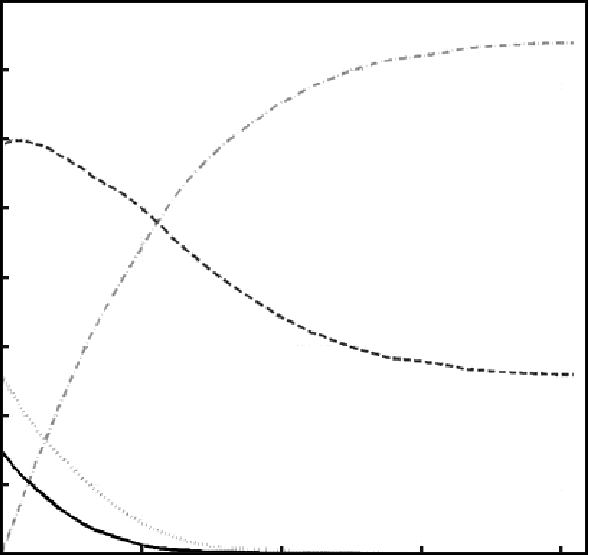
\includegraphics[width=6cm]{img/chap5/brill2_refait}};

\draw[legende] (-1.1,-1.1) rectangle (2.9,-2.7);

\draw (-0.4,-1.3) node[anchor=west, font=\footnotesize] {fausse égalité};
\draw (-0.4,-1.7) node[anchor=west, font=\footnotesize] {fausse différenciation};
\draw (-0.4,-2.1) node[anchor=west, font=\footnotesize] {faux ordonnancement};
\draw (-0.4,-2.5) node[anchor=west, font=\footnotesize] {décision correcte};

\draw[very thick, help lines, densely dashed] (-1,-1.3) -- (-0.4,-1.3);
\draw[thick, help lines, densely dotted] (-1,-1.7) -- (-0.4,-1.7);
\draw[very thick] (-1,-2.1) -- (-0.4,-2.1);
\draw[very thick, densely dashed] (-1,-2.55) -- (-0.4,-2.55);

\node[below=0.3cm,rotate=90] at (-4,0.5) {Proportions};
\node[anchor=east] at (-2.9,-2.8) {0};
\node[anchor=east] at (-2.9,-2.1) {0,1};
\node[anchor=east] at (-2.9,-1.4) {0,2};
\node[anchor=east] at (-2.9,-0.7) {0,3};
\node[anchor=east] at (-2.9,0) {0,4};
\node[anchor=east] at (-2.9,0.7) {0,5};
\node[anchor=east] at (-2.9,1.4) {0,6};
\node[anchor=east] at (-2.9,2.1) {0,7};
\node[anchor=east] at (-2.9,2.8) {0,8};

\node at (0,-3.5) {$\Delta \mathit{OVQM}$};
\node[anchor=north] at (-3,-2.8) {0};
\node[anchor=north] at (-1.6,-2.8) {0,1};
\node[anchor=north] at (-0.1,-2.8) {0,2};
\node[anchor=north] at (1.3,-2.8) {0,3};
\node[anchor=north] at (2.7,-2.8) {0,4};


% \end{tikzpicture}\end{tikzpicture}}
	\caption{Exemples de résultats obtenus par Brill~\cite{brill-spic}.}
	\label{fig:brill}
\end{figure}

Les auteurs proposent également une classification des erreurs d'un critère. Ces erreurs correspondent aux cas où le critère objectif et le test subjectif fournissent des conclusions différentes sur une paire de séquences. Trois cas sont possibles, que les auteurs classent dans l'ordre de gravité croissante : la fausse égalité est le cas où les deux mesures subjectives sont différentes mais où les notes objectives sont égales ; la fausse différenciation est le cas où les deux mesures subjectives sont égales mais où les notes objectives sont différentes ; le faux ordonnancement est le cas où les notes objectives sont dans l'ordre opposé des mesures subjectives.

La figure~\ref{fig:brill2} présente les proportions de ces erreurs pour le PSNR calculé sur les séquences de la première campagne de VQEG~\cite{vqeg-frtv1}. Cette méthode est intéressante dans la mesure où elle permet une visualisation directe de la précision d'un critère. De plus, elle fournit un indice de confiance sur la différence entre deux notes objectives. En effet, elle montre qu'en-dessous d'un certain seuil, il y a plus de chances que cette différence soit due à une erreur du critère plutôt qu'à la réalité.


\subsubsection{Mesure de monotonie}
Pour rendre compte de la monotonie de la relation entre les mesures subjectives et les notes objectives, le coefficient de corrélation linéaire~\cite{pearson-rslpt}, noté cc, est utilisé :
\begin{equation}
\text{cc} = \frac{\frac{1}{N_n}\sum\limits_{i=1}^{N_n} (\MS(i) - \mu_{\MS})\cdot (\MSP(i) - \mu_{\MSP})}{\sigma_{\MS} \cdot \sigma_{\MSP}}
\end{equation}
%
avec $\mu_{\MS}$ et $\mu_{\MSP}$ les moyennes respectives des distributions $\MS$ et $\MSP$ et $\sigma_{\MS}$ et $\sigma_{\MSP}$ les écarts-type respectifs des distributions $\MS$ et $\MSP$. Ce coefficient mesure la qualité de la dépendance linéaire entre les deux variables $\MS$ et $\MSP$. Il est compris entre -1 et 1. Plus il est proche de ces extrémités, plus la dépendance linéaire est forte.

En plus des indicateurs de performance fournis par VQEG, nous ajoutons le coefficient de corrélation de rang~\cite{spearman-ajp}, noté ccr :
\begin{equation}
\text{ccr} = 1 - \dfrac{6\times\sum\limits_{i=1}^{N_n} \left[r(\MS(i)) - r(\MSP(i))\right]^2}{N_n^3 - N_n}
\end{equation}
%
avec $r(X)$ le rang de l'élément $X$. Ce coefficient reflète, pour l'ensemble des séquences, les différences entre le classement d’une séquence dans l’ensemble des notes objectives et son classement dans l’ensemble des mesures subjectives.


\subsubsection{Mesure de cohérence}
La dernière mesure caractérise la cohérence du critère évalué. Elle évalue la proportion de mesures subjectives de qualité trop mal prédites par le critère objectif de qualité. Il s'agit de l'\emph{outlier ratio}, noté or. Il est égal au rapport entre le nombre de configurations mal évaluées $N_e$ et le nombre total de mesures $N_n$ :
\begin{equation}
\text{or} = \frac{N_{e}}{N_n}. \label{eq:or}
\end{equation}
%
Une configuration $i$ est considérée comme mal évaluée si le critère suivant est vérifié ($\IC$ est l'intervalle de confiance) :
\begin{equation}
|\MS(i) - \MSP(i)| > 2\times\IC(i).
\end{equation}
%
Plus ce rapport est faible, plus le critère est cohérent.


\subsubsection{Discussion}
Il existe d'autres mesures de performance. Citons par exemple l'erreur absolue moyenne, le coefficient de Kappa~\cite{cohen-kappa} utilisé dans le cas d'une échelle d'évaluation discrète ou encore les coefficients de corrélation utilisés par VQEG dans sa première campagne d'évaluation de critères objectifs~\cite{vqeg-frtv1}. En dehors des mesures plus originales de Brill~\cite{brill-spic}, la sélection présentée ici est classique mais complète. En effet, il est courant de constater l'usage d'une seule de ces mesures et de conclure sur les performances d'un critère à partir de seulement quelques chiffres. Pourtant, ces mesures sont importantes dans l'exploitation des résultats obtenus par un critère, et chacune apporte sa contribution à l'évaluation globale des performances. Sauf mention contraire, pour chaque critère que nous évaluerons par la suite, nous donnerons les valeurs des cinq mesures cc, ccr, reqm, reqmp et or.

Par ailleurs, nous regrettons que VQEG ait en partie changé de mesures de performances entre ses deux campagnes d'évaluation de critères pour la télévision. Cela ne permet pas de comparer les deux ensembles de critères objectifs, de les classer et de considérer les meilleurs à leur juste valeur.


\subsection{Signifiance de la différence entre deux mesures de performance}
Plus l'ensemble de séquences sur lequel les mesures de performance sont calculées est grand, plus celles-ci sont précises. Or, le nombre de séquence étant souvent restreint, la précision des mesures de performance est limitée. Pour savoir si la différence entre deux mesures est due à de réelles différences de performance entre les critères et non pas à cette imprécision, il existe des outils de calcul de signifiance. VQEG les a récemment introduits dans ces études~\cite{vqeg-MMtestplan,vqeg-hdtvtestplan}. Ils sont par contre encore peu utilisés par le monde universitaire. Leur intérêt est pourtant évident car ils permettent de comparer les mesures de performance sur des critères statistiques chiffrés.

Il y a deux moyens de tester la signifiance d'une différence entre deux mesures. Le premier est calculer directement son intervalle de confiance. La différence est alors considérée comme significative si les bornes de cet intervalle sont du même signe. La seconde est de comparer les intervalles de confiance des deux mesures. S'ils se chevauchent, c'est que la différence n'est pas significative. Usuellement, tous ces tests se font avec un niveau de signification de 0,05. Il s'agit donc d'intervalles de confiance à 95\%.


\subsubsection{Différence entre racines carrées de l'erreur quadratique moyenne}
Pour évaluer la différence entre deux reqm $\mathit{reqm}_1$ et $\mathit{rqm}_2$ tels que $\mathit{reqm}_1 > \mathit{reqm}_2$ et qu'ils soient calculés respectivement sur $N_1$ et $N_2$ paires d'éléments, nous considérons le rapport :
\begin{equation}
\zeta = \frac{\mathit{reqm}_1}{\mathit{reqm}_2}.
\end{equation}
%
Le test utilise la table de la distribution F avec pour paramètres le niveau de signification de 0,05 et les nombres de degrés de liberté de chaque écarts $N_1 - 1$ et $N_2 - 1$. La table fournit la valeur $F_{N_1-1;N_2-1}$ à comparer à $\zeta$. Si $\zeta > F_{N_1-1;N_2-1}$, alors la différence entre $\mathit{reqm}_1$ et $\mathit{reqm}_2$ est considérée comme statistiquement significative.

À l'usage, cette méthode se montre particulièrement critique. Par exemple, sur une base de séquences comme celle de l'annexe~\ref{annex:base}, nous avons $F_{\text{167};\text{167}}$ = 1,2908. Pour être statistiquement différents, les deux racines carrées de l'erreur quadratique moyenne doivent donc être différentes de près de 30\%. Cela montre bien l'importance de la taille de la base de séquences. Pourtant, des conditions aussi critiques rendent difficile l'obtention de différences significatives, ce qui peut expliquer le peu d'utilisation de ces outils dans la littérature. En effet, qui d'autre que VQEG a les moyens de créer une quantité de données suffisantes pour atteindre une telle précision ?


\subsubsection{Différence entre coefficients de corrélation}
Mesurer les performances d'un critère objectif sur une base de séquence est une première étape. La seconde est de les comparer avec celles d'autres critères. Pour cela, il est possible de déterminer si la différence entre deux coefficients de corrélation linéaire est significative ou non.

Considérons deux coefficients de corrélation $\mathit{cc}_1$ et $\mathit{cc}_2$, calculés respectivement sur $N_1$ et $N_2$ paires d'éléments. La première étape est de transformer $\mathit{cc}_1$ et $\mathit{cc}_2$ par la transformation en Z de Fisher~\cite{fisher-z} :
\begin{equation}
z_1 = \frac{1}{2} \ln\left(\frac{1+\mathit{cc}_1}{1-\mathit{cc}_1}\right) \text{ et } z_2 = \frac{1}{2} \ln\left(\frac{1+\mathit{cc}_2}{1-\mathit{cc}_2}\right).
\end{equation}
%
Cette transformation permet de passer d'une distribution non normale à une distribution normale dont l'écart-type est connu et vaut :
\begin{equation}
\sigma_z = \frac{1}{\sqrt{N_n-3}}
\end{equation}
%
avec $N_n$ le nombre d'éléments. Dans notre cas, nous calculons l'écart-type de la différence $z_1-z_2$ :
\begin{equation}
\sigma_{z_1-z_2} = \sqrt{\frac{1}{N_1-3} +\frac{1}{N_2-3}}.
\end{equation}
%
L'étape suivante est de calculer les bornes $z_b$ et $z_h$ de cet écart-type :
\begin{equation}
\begin{array}{c}
z_b = z_1-z_2 - 1,96\times \sigma_{z_1-z_2}\\
z_h = z_1-z_2 + 1,96\times \sigma_{z_1-z_2}.
\end{array}
% z_b = z_1-z_2 - 1,96\times \sigma_{z_1-z_2} \text{ et } z_h = z_1-z_2 + 1,96\times \sigma_{z_1-z_2}.
\end{equation}
%
Ces bornes sont ensuite converties par la transformation en Z inverse :
\begin{equation}
\mathit{cc}_b = \frac{e^{2z_b}-1}{e^{2z_b}+1} \text{ et } \mathit{cc}_h = \frac{e^{2z_h}-1}{e^{2z_h}+1}.
\end{equation}
%
L'intervalle de confiance de la différence des coefficients de corrélation est donc :
\begin{equation}
\mathit{cc}_b \leqslant \mathit{cc}_1 - \mathit{cc}_2 \leqslant \mathit{cc}_h.
\end{equation}
%
Le test final vérifie le signe des deux bornes. Si elles n'ont pas le même signe, cela signifie qu'il reste une incertitude sur la différence des corrélations. Par contre, si elles sont du même signe, cela signifie que la différence est significative. À titre d'illustration, la figure~\ref{fig:plotICcc} présente l'évolution des bornes haute et basse en fonction du coefficient de corrélation considéré. Trois valeurs de $N_n$ y sont utilisées.

\begin{figure}[htbp]
	\centering
	\begin{tikzpicture}[scale=6]
	\node at (-0.02,-0.02) {0};
	\draw[->] (0,0) -- (1.1,0) node[right] {cc};
	\draw[->] (0,0) -- (0,1.1) node[above] {bornes};
	\draw[dotted] (0,0) -- (1,1);

	\foreach \x in {0.2,0.4,0.6,0.8,1}
	{
		\draw (\x,0) -- (\x,-0.01) node[anchor=north] {\x};
		\draw (0,\x) -- (-0.01,\x) node[anchor=east] {\x};
	}

	\draw plot[smooth] file {plot/chap5/lhCC42};
	\draw plot[smooth] file {plot/chap5/lbCC42};
	\draw[densely dashed] plot[smooth] file {plot/chap5/lhCC168};
	\draw[densely dashed] plot[smooth] file {plot/chap5/lbCC168};
	\draw[loosely dashed] plot[smooth] file {plot/chap5/lhCC384};
	\draw[loosely dashed] plot[smooth] file {plot/chap5/lbCC384};

	\draw[legende] (0.1,0.8) rectangle (0.45,1.05);
	\draw[thick] (0.12,1) -- (0.22,1) node[anchor=west] {$N_n$=42};
	\draw[thick,densely dashed] (0.12,0.93) -- (0.22,0.93) node[anchor=west] {$N_n$=168};
	\draw[thick,loosely dashed] (0.12,0.85) -- (0.22,0.85) node[anchor=west] {$N_n$=384};

	\node at(0.5,0.1) {$cc_b$};
	\node at(0.1,0.5) {$cc_h$};
\end{tikzpicture}

	\caption{Bornes haute $cc_h$ et basse $cc_b$ d'un coefficient de corrélation cc pour plusieurs valeurs du nombre d'éléments $N_n$.}
	\label{fig:plotICcc}
\end{figure}


\subsubsection{Différence entre \emph{outlier ratio}}
L'\emph{outlier ratio} peut être décrit par une distribution binomiale de paramètres $(p, 1-p)$ avec $p$ définie par la relation~\ref{eq:or}. Cette distribution est caractérisée par sa moyenne $p$ et son écart-type :
\begin{equation}
\sigma_p = \sqrt{\frac{p(1-p)}{N_n}}
\end{equation}
%
avec $N_n$ le nombre total de mesures. Pour $N_n$ > 30, la distribution binomiale est approchée par une distribution gaussienne. L'intervalle de confiance à 95\% de l'\emph{outlier ratio} est donc :
\begin{equation}
\IC_{or} = \pm 2\sigma_p.
\end{equation}
%
Deux \emph{outlier ratios} sont considérés comme statistiquement différents si leurs intervalles de confiance ne se chevauchent pas.


\section{Évaluation du critère de qualité vidéo VSSIM}
Nous ne reviendrons pas sur la présentation technique du critère que nous avons faite à la section~\ref{ssec:ssim}. La figure~\ref{fig:VSSIM} de la page~\pageref{fig:VSSIM} en présente la structure originale. %Rappelons juste que, comme son nom l'indique, ce critère utilise l'index de qualité pour images fixes SSIM de Wang et Bovik~\cite{wang-ssim}.


\subsection{Mise en \oe uvre du critère}
Pour la mise en application de ce critère sur les séquences de notre base, plusieurs adaptations ont été nécessaires. La figure~\ref{fig:vssimMod} présente la structure modifiée du critère par rapport à la structure originale de la figure~\ref{fig:VSSIM}. Comme base de travail, nous avons utilisé une fonction logicielle fournie par l'auteur. Elle calcule une carte de mesures SSIM locales entre deux images. La taille des fenêtres locales où sont calculées ces mesures est paramétrable.

\begin{figure}[htbp]
	\centering
	\begin{tikzpicture}[text centered, text width=2cm,node distance=3cm]% \begin{tikzpicture}
\node[text width=1.4cm] (ref) {vidéo de référence};
\node[right of=ref] (refBis) {};
\node[action,right of=refBis,node distance=1.8cm] (convRef) {conversion vers 4$:$4$:$4};
\node[below of=ref,node distance=1cm] (tmp) {};
\node[below of=tmp,node distance=2cm,text width=1.4cm] (deg) {vidéo dégradée};
\node[action,right of=deg,node distance=2.4cm] (convDeg) {conversion vers 4$:$4$:$4};

\node[action, right of=convDeg,text width=1.5cm,node distance=2.4cm] (ssim) {calcul SSIM};
\node[action, right of=ssim,node distance=3.1cm] (cumulImage) {cumul sur l'image $i$};
\node[action, right of=cumulImage,node distance=2.8cm] (cumulSeq) {cumul sur la séquence};
\node[right of =cumulSeq,text width=1.2cm,node distance=2.15cm] (vssim) {VSSIM};
\node[action, above of=cumulImage,node distance=2cm] (calculw) {calcul de $w_{\mathit{ij}}$};
\node[action, right of=calculw,node distance=2.8cm] (calculW) {calcul de $W_i$};

\path[fleche] (ref) -- (convRef);
\path[fleche] (convRef) -| (calculw) node[right=-0.2cm, pos=0.7] {luminance};
\path[fleche] (calculw) -- (cumulImage) node[right=-0.8cm,pos=0.5] {$w_{\mathit{ij}}$};
\path[fleche] (calculW) -- (cumulSeq) node[right=-0.8cm,pos=0.5] {$W_i$};
\path[fleche] (deg) -- (convDeg);
\path[fleche] (convDeg) -- (ssim);
\path[fleche] (ssim) -- (cumulImage) node[below,pos=0.5] {$\text{SSIM}_{\mathit{ij}}$};
\path[fleche] (cumulImage) -- (cumulSeq) node[below,pos=0.5] {$Q_i$};
\path[fleche] (cumulSeq) -- (vssim);
\path[fleche] (convRef) -- (ssim);
\path[fleche] (convRef) -| (calculW) node[right,pos=0.7] {vecteurs de mouvement};

% \end{tikzpicture}
\end{tikzpicture}
	\caption{Structure adaptée du critère de qualité vidéo VSSIM pour sa mise en \oe uvre.}
	\label{fig:vssimMod}
\end{figure}

Pour effectuer le cumul sur les composantes, nous devons disposer des matrices $Y$, $C_b$ et $C_r$ correspondantes et de même taille. Or, les séquences d'origine sont au format 4$:$2$:$0 et 4$:$2$:$2. Une conversion au format 4$:$4$:$4 est d'abord effectuée. Ceci est réalisé en sur-échantillonnant les composantes $C_b$ et $C_r$ d'un facteur deux dans une ou deux directions suivant le format d'origine. Le sur-échantillonnage est effectué en recopiant la valeur du plus proche voisin de chaque pixel d'origine.

Les auteurs préconisent de ne pas utiliser toutes les fenêtres glissantes locales et d'en considérer qu'une sous-partie. Cependant, nous avons effectué le calcul sur l'ensemble des fenêtres car l'étape de génération des cartes SSIM n'est pas la plus complexe. La gestion des vidéos TVHD est elle-même très gourmande en ressources et nécessite un temps bien supérieur. Le gain engendré par l'utilisation d'une sous-partie de ces fenêtres serait donc minime. De plus, alors que les auteurs utilisent des fenêtres 8\texttimes8, nous utilisons des fenêtres de taille 16\texttimes16. Cela permet de simplifier en partie les calculs.

Enfin, nous ne disposons pas des vecteurs de mouvement de chaque fenêtre 16\texttimes16 de chaque image des séquences. Par contre, nous disposons du vecteur moyen des fenêtres de l'image centrale d'un groupe de cinq images successives. Ils sont issus de la méthode de classification spatio-temporelle d'une séquence vidéo présentée à la section~\ref{sec:methodeClassifST}. Nous avons donc décidé d'utiliser ce vecteur de mouvement moyen pour chacune des cinq fenêtres correspondantes. C'est l'approximation la plus grossière dans l'adaptation du critère. Néanmoins, nous considérons qu'elle ne perturbe pas les résultats de manière significative. En effet, notre méthode d'estimation de mouvement est particulièrement précise car elle s'appuie sur une durée d'estimation plus importante. %Ainsi, les vecteurs de mouvement calculés de cette manière sont précis et


\subsection{Performances sur une base de séquences TVSD}
Les auteurs~\cite{wang-vqasdm} ont évalué les performances de ce critère de qualité vidéo sur la base de séquences au format TVSD de VQEG~\cite{vqeg-frtv1}. Cela leur permet de les comparer avec celles obtenues par les autres critères de cette campagne d'évaluation. Le tableau~\ref{tab:perfVSSIMsurVQEG} présente ces performances. À titre de comparaison, nous y trouvons également les meilleures performances obtenues lors de cette campagne. Elles sont à mettre au crédit du critère de KPN. Rappelons cependant qu'elles ne sont pas significativement supérieures à celles des autres critères. Le coefficient de corrélation cc1 est calculé entre les notes objectives et les mesures subjectives après une régression basée sur la minimisation de l'erreur de prédiction. Le coefficient de corrélation cc2 est calculé après une régression non linéaire. Ces mesures de performance sont fournies par VQEG~\cite{vqeg-frtv1}.

\begin{table}[htbp]
\centering
\begin{tabular}{ccccc}\toprule
\strong{critère}	&	\strong{cc1}	& \strong{cc2}	& \strong{ccr} 	& \strong{or}	\\ \toprule
VSSIM					& 0,864				& 0,849				& 0,812				& 0,578			\\ \midrule
KPN						& 0,845 				& 0,827 				& 0,803				& 0,578			\\ \bottomrule
\end{tabular}
\caption{Performances de VSSIM sur la base de séquences TVSD de VQEG~\cite{vqeg-frtv1}.}
\label{tab:perfVSSIMsurVQEG}
\end{table}

Les résultats obtenus par VSSIM sont numériquement supérieurs à ceux des autres critères évalués lors de cette campagne. Malheureusement, les auteurs n'indiquent pas si la différence est significative ni le nombre exact de séquences utilisées. Cependant, pour que le coefficient de corrélation obtenu par VSSIM soit significativement différent de celui de KPN, il faudrait qu'ils soient évalués sur plus de 1500 séquences chacun. Or, VQEG n'a utilisé au maximum que 384 séquences. VSSIM n'est donc pas sensiblement meilleur que les autres critères de cette campagne d'évaluations.


\subsection{Performances sur une base de séquences haute définition}
Nous avons calculé les performances de VSSIM sur l'ensemble des séquences dégradées de l'annexe~\ref{annex:base}. Les DMOS prédits sont obtenus à partir des mesures VSSIM par une fonction d'ajustement de type psychométrique qui adapte la dynamique [0 ; 1] du critère à celle de notre échelle de qualité [0 ; 100]. Le tableau~\ref{tab:perfVSSIM} présente les performances obtenues. Deux types d'écran différents ont été utilisés. $N_n$ est le nombre de séquences sur lesquelles les performances sont calculées.

\begin{table}[htbp]
\centering
\begin{tabular}{cccccccc}\toprule
\strong{écran}	& $N_n$	& \strong{cc}	& \strong{ccr}	& \strong{reqm} 	& \strong{reqmp}	& \strong{or} \\ \toprule
LCD						& 168	& 0,7900 			& 0,7305			& 11,2713			& 1,8406				& 0,5476			\\ \midrule
CRT						& 84		& 0,5640 			& 0,5032			& 12,7042			& 2,1251				& 0,6786			\\ \bottomrule
\end{tabular}
\caption{Performances de VSSIM sur les séquences haute définition de la base de l'annexe~\ref{annex:base}.}
\label{tab:perfVSSIM}
\end{table}

L'intervalle de confiance sur la différence des deux coefficients de corrélation est [0,1653 ; 0,6035]. Cela montre qu'ils sont significativement différents. Par contre, le rapport des reqm vaut 1,1271 et $F_{167;83}$ = 1,3819 donc les reqm ne sont pas significativement différentes. Les intervalles de confiance sur les \emph{outlier ratio} sont respectivement [0,4708 ; 0,6244] et [0,5767 ; 0,7805] pour les types d'écrans LCD et CRT. La différence entre les deux est donc assez importante. Le type d'écran a donc une influence sur les performances de VSSIM, alors qu'il ne tient pas compte du type d'écran utilisé. Les figures~\ref{fig:nuageVSSIMLCD} et~\ref{fig:nuageVSSIMCRT} respectivement présentent les DMOS prédits en fonction des DMOS subjectifs mesurés sur écran LCD et CRT. Les droites en pointillés correspondent à l'égalité entre les DMOS et les DMOSP. Le calcul de DMOS peut parfois arriver à des valeurs négatives, si la séquence de référence est moins bien évaluée que la séquence dégradée. C'est le cas pour certaines séquences de la figure~\ref{fig:nuageVSSIMCRT}.

\begin{figure}[htbp]
	\centering
	\subfloat[\label{fig:nuageVSSIMLCD} DMOS prédits par le critère VSSIM en fonction des DMOS subjectifs mesurés sur écran LCD.]{\begin{tikzpicture}[only marks, scale=0.07]
	\pgfsetplotmarksize{1cm}
	\draw plot[mark=+] file {plot/chap5/DMOSLCD-DMOSpVSSIM.txt};
	\draw[->] (0,0) -- coordinate (x axis) (85,0);
	\draw[->] (0,0) -- coordinate (y axis) (0,85);
	\foreach \x in {0,20,40,60,80} \draw (\x cm,1cm) -- (\x cm,-1cm) node[anchor=north] {\x};
	\foreach \y in {0,20,40,60,80} \draw (1cm,\y cm) -- (-1cm,\y cm) node[anchor=east] {\y};
	\node[below=0.5cm] at (x axis) {DMOS prédits};
	\node[left=0.9cm,rotate=90] at (0,50) {DMOS};
	\draw[dotted] (0,0) -- (80,80);
\end{tikzpicture}}\hfill
	\subfloat[\label{fig:nuageVSSIMCRT} DMOS prédits par le critère VSSIM en fonction des DMOS subjectifs mesurés sur écran CRT.]{\begin{tikzpicture}[only marks, scale=0.07]
	\pgfsetplotmarksize{1cm}
	\draw plot[mark=+] file {plot/chap5/DMOSCRT-DMOSpVSSIM.txt};
	\draw[->] (0,-20) -- coordinate (x axis) (85,-20);
	\draw[->] (0,-20) -- coordinate (y axis) (0,65);
	\foreach \x in {0,20,40,60,80} \draw (\x cm,-19) -- (\x cm,-21) node[anchor=north] {\x};
	\foreach \y in {-20,0,20,40,60} \draw (1cm,\y cm) -- (-1cm,\y cm) node[anchor=east] {\y};
	\node[below=0.5cm] at (x axis) {DMOS prédits};
	\node[left=0.9cm,rotate=90] at (0,30) {DMOS};
	\draw[dotted] (0,0) -- (60,60);
\end{tikzpicture}
}\\
  \caption{DMOS prédits par le critère de qualité vidéo VSSIM en fonction des DMOS subjectifs mesurés sur écran LCD et CRT.}
\end{figure}

Les performances obtenues sont globalement peu satisfaisantes. La corrélation linéaire n'est pas bonne pour les deux types d'écran, révélant la monotonie médiocre du critère. Ceci est confirmé par la dispersion des points visible sur les figures~\ref{fig:nuageVSSIMLCD} et~\ref{fig:nuageVSSIMCRT}. Les erreur de l'ordre d'un dixième de la dynamique montrent quand à eux que la précision est assez moyenne. Les \emph{outlier ratio} confirment la tendance générale avec des valeurs indiquant une cohérence médiocre. De plus, la différence de corrélation entre VSSIM sur TVSD et VSSIM sur TVHD est significative. Cela indique que le critère est moins performant dans l'estimation de la qualité de la TVHD que dans celle de la TVSD.


\section{Évaluation du critère de qualité vidéo VQM} \label{ssec:evalVQM}
Le critère VQM \emph{(Video quality metric)} est proposé par Wolf et Pinson~\cite{wolf-vqmtech} du NTIA \emph{(National telecommunications and information administration)}. C'est le critère ayant obtenu les meilleurs résultats lors de la seconde campagne d'évaluation de critères objectifs de qualité vidéo réalisée par VQEG en 2003~\cite{vqeg-frtv2}. Il a par la suite fait partie des quatre critères retenus en vue d'une normalisation~\cite{itu-j144}. Les auteurs fournissent un logiciel permettant de mesurer directement la qualité de séquences avec le critère, ce qui permet d'éviter les adaptations comme celles réalisées pour VSSIM.


\subsection{Présentation du critère}
La figure~\ref{fig:vqmGlobal} présente la structure globale du critère. Dans la terminologie de VQM, un modèle est un algorithme spécifiquement optimisé pour atteindre une corrélation maximale entre les données objectives et subjectives dans différentes situations. Les cinq modèles existants sont :
\begin{itemize}
\item \emph{Television}, optimisé pour la télévision ;
\item \emph{Videoconferencing}, optimisé pour la vidéoconférence ;
\item \emph{General}, optimisé pour une utilisation générique, c'est-à-dire avec une large gamme de qualité et de débit ;
\item \emph{Developer}, optimisé pour une large gamme de qualité et de débit avec une contrainte de faible complexité ;
\item \emph{Peak-signal-to-noise-ratio}, utilisant le PSNR comme mesure de qualité.
\end{itemize}

\begin{figure}[htbp]
	\centering
	\begin{tikzpicture}[text centered,text width=2cm,node distance=1.5cm]% \begin{tikzpicture}[text centered,text width=2cm] % schéma schéma du critère VQM
\node (ref) {vidéo de référence};
\node[action,right of=ref,node distance=3cm] (codage) {codage};
\node[action,right of=codage,node distance=3cm] (decodage) {décodage};
\node[right of=decodage,node distance=3cm] (deg) {vidéo dégradée};

\node[action,below of=ref] (calibRef) {calibrage};
\node[action,below of=deg] (calibDeg) {calibrage};
\node[action,text width=3cm,below of=calibRef] (caracRef) {extraction de caractéristiques};
\node[action,text width=3cm,below of=calibDeg] (caracDeg) {extraction de caractéristiques};

\node[right of=caracRef,node distance=4.5cm] (tmp) {};
\node[action,text width=5cm,below of=tmp,node distance=1.2cm] (param) {calcul de paramètres de qualité};
\node[action,below of=param,text width=2.5cm,node distance=1.2cm] (modele) {modèle VQM};
\node[below of=modele,text width=2.5cm,node distance=1.2cm] (vqm) {note de qualité};

\path[fleche] (ref) -- (codage);
\path[fleche] (codage) -- (decodage);
\path[fleche] (decodage) -- (deg);
\path[fleche] (ref) -- (calibRef);
\path[fleche] (deg) -- (calibDeg);
\path[fleche] (calibRef) -- (caracRef);
\path[fleche] (calibDeg) -- (caracDeg);
\path[fleche] (caracRef) |- (param);
\path[fleche] (caracDeg) |- (param);
\path[fleche] (param) -- (modele);
\path[fleche] (modele) -- (vqm);

% \end{tikzpicture}
\end{tikzpicture}
	\caption{Structure globale du critère de qualité vidéo VQM~\cite{wolf-vqmtech}.}
	\label{fig:vqmGlobal}
\end{figure}

La première étape de calibrage permet de préparer les séquences à être comparées. Celle-ci estime :
\begin{itemize}
\item l'alignement et l'éventuelle correction spatiaux entre les deux séquences ;
\item l'estimation de la région spatiale d'intérêt pour l'extraction des caractéristiques ;
\item l'estimation et l'éventuelle correction du contraste et de la luminosité perçue ;
\item l'alignement et l'éventuelle correction temporels entre la séquence d'origine et la séquence dégradée.
\end{itemize}

VQM calcule ensuite des caractéristiques locales extraites de la séquence de référence et de celle à évaluer avant de les comparer. L'extraction des caractéristiques se fait par régions spatio-temporelles élémentaires. Une telle région est un ensemble de pixels défini par ses deux dimensions spatiales $(\Delta h,\Delta v)$ et sa dimension temporelle $\Delta t$. La figure~\ref{fig:vqmTube} en présente la structure. Par défaut, VQM utilise des régions de taille $(\Delta h,\Delta v,\Delta t)=($8,8,6$)$, mais ces valeurs peuvent différer d'un modèle à l'autre. Le critère utilise six caractéristiques. Deux caractérisent l'activité spatiale, une troisième les distorsions dans les composantes chromatiques, une quatrième le contraste local, une cinquième la quantité d'information temporelle et enfin la sixième est le produit de la caractéristique du contraste local et de celle de l'information temporelle.

\begin{figure}[htbp]
	\centering
	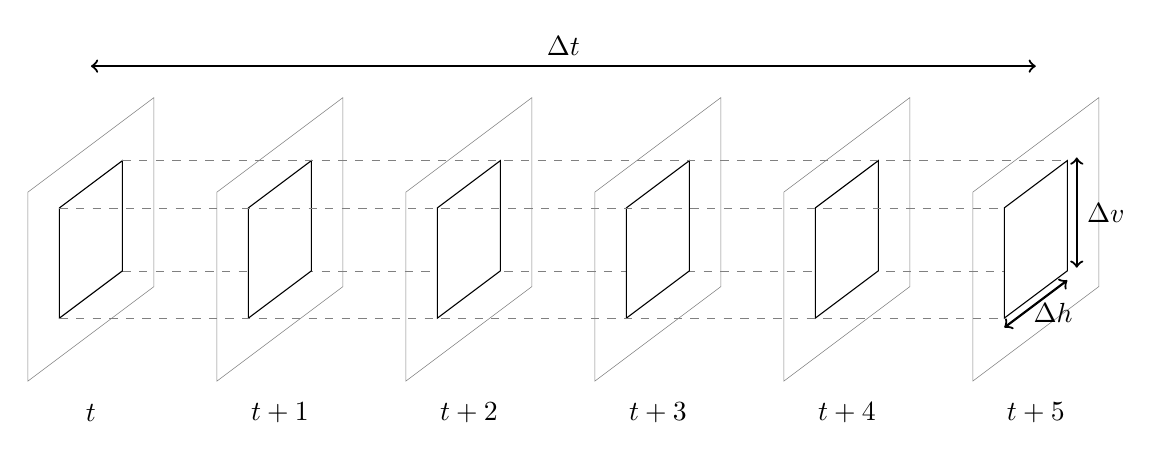
\begin{tikzpicture}[scale=0.4] % schéma du tube VQM dans une image

\draw[dashed,help lines] (3,3.5) -- (31,3.5);

\foreach \j in {0,3,6,9,12,15} % grille sur les autres images
{
	\draw[help lines] (2*\j,0) -- (4+2*\j,3) -- (4+2*\j,9) -- (2*\j,6) -- cycle;
	\filldraw[fill=white] (2*\j+1,2) -- (3+2*\j,3.5) -- (3+2*\j,7) -- (2*\j+1,5.5) -- cycle;
}

\path[thick,draw,<->] (33.3,3.6) -- (33.3,7.1) node[right,pos=0.5] {$\Delta v$};
\path[thick,draw,<->] (31,1.7) -- (33,3.2) node[right,pos=0.3] {$\Delta h$};
\path[thick,draw,<->] (2,10) -- (32,10) node[above,pos=0.5] {$\Delta t$};
\draw (2,-1) node{$t$};

\foreach \j in {1,2,3,4,5} % grille sur les autres images
{
	\draw (2+6*\j,-1) node{$t+\j$};
}

\draw[dashed,help lines] (1,5.5) -- (31,5.5);
\draw[dashed,help lines] (1,2) -- (31,2);
\draw[dashed,help lines] (3,7) -- (33,7);

\end{tikzpicture}

	\caption{Tube d'extension spatio-temporelle ($\Delta h$,$\Delta v$,$\Delta t$) utilisé dans VQM~\cite{wolf-vqmtech}.}
	\label{fig:vqmTube}
\end{figure}

Des fonctions sont utilisées pour mesurer les distorsions de la vidéo dégradée par rapport à la vidéo originale en fonction de l'évolution des caractéristiques. Il s'agit de différentes fonctions de comparaison, de calcul de distance, de cumul et de seuillage. La combinaison des caractéristiques et des fonctions fournit des paramètres de gain ou de perte de qualité en grande quantité. Cela permet de couvrir une large gamme de contextes et explique la diversité des modèles proposés. Chaque modèle consiste ensuite en une combinaison linéaire d'une sélection de fonctions appliquées aux caractéristiques. Les pondérations de ces combinaisons sont obtenues par optimisation. La sélection des fonctions est faire de sorte à retenir les plus pertinentes. Enfin, chaque modèle produit une valeur comprise entre 0 et 1. La valeur nulle correspond à la perception d'aucune distorsion, alors que la valeur un correspond à la perception maximale de distorsions.

Un logiciel est fourni par le laboratoire NTIA pour l'utilisation de VQM à des fins de recherche scientifique. Nous l'avons utilisé pour obtenir des notes objectives de qualité pour les séquences de la base présentée à l'annexe~\ref{annex:base}. Le contexte visé étant la télévision haute définition, nous avons utilisé le modèle \emph{Television}. Le calibrage est fait automatiquement par le logiciel. Cette étape a parfois tendance à réduire la durée des séquences, car la durée totale doit être un multiple de la taille d'une région spatio-temporelle. Ainsi, les séquences de douze secondes présentes dans la base sont réduites à dix secondes. De même, le calibrage réduit parfois les séquences de quelques pixels sur les bords pour éliminer les éléments qui ne présentent pas d'intérêt.


\subsection{Performances sur une base de séquences TVSD}
VQM a été évalué lors des deux campagnes effectuées par VQEG. Nous considérons ici les performances obtenues lors de la seconde campagne~\cite{vqeg-frtv2}. Celles-ci ont été calculées à partir de 64 séquences dégradées pour le format PAL et 63 pour le format NTSC. Le modèle \emph{General} fut alors utilisé. Le tableau~\ref{tab:perfVQMsurVQEG} présente ces résultats.

\begin{table}[htbp]
\centering
\begin{tabular}{ccccc} \toprule
\strong{format}	&	$N$	& \strong{cc}	& \strong{ccr}	& \strong{or}	\\ \toprule
PAL						& 64		& 0,886			& 0,879			& 0,31				\\ \midrule
NTSC					& 63		& 0,938 			& 0,936 			& 0,46				\\ \bottomrule
\end{tabular}
\caption{Performances du critère objectif de qualité vidéo VQM sur la base de séquences TVSD de VQEG~\cite{vqeg-frtv2}.}
\label{tab:perfVQMsurVQEG}
\end{table}

La différence entre les coefficients de corrélation des deux formats n'est pas significative. Cela n'est pas très surprenant étant donné leur proximité et le faible nombre de séquences sur lesquelles ils ont été évalués. Néanmoins, les résultats obtenus par VQM sur l'ensemble de séquences au format NTSC sont très bons en termes de corrélation. La monotonie de la relation entre le modèle et les DMOS est très forte. Pourtant, l'\emph{outlier ratio} reste assez élevé. Il est sensiblement meilleur pour le format PAL, alors que les corrélations sont plus faibles. Le modèle s'avère donc plus précis mais moins monotone dans ce contexte.

Suivant le format testé, la différence avec VSSIM peut être significative. En effet, la comparaison entre les coefficients de corrélation de VSSIM et de VQM au format PAL n'est pas significative. Elle l'est en comparant avec VQM au format NTSC. Nous constatons l'inverse pour les \emph{outlier ratio}. La différence est significative avec le format PAL, mais pas avec le format NTSC. Malheureusement, nous ne disposons pas de la distinction des formats pour les résultats de VSSIM, ce qui nous empêche de mener plus en avant cette comparaison.


\subsection{Performances sur une base de séquences haute définition}
Nous avons calculé les mêmes mesures de performances que pour VSSIM sur la base de séquences haute définition présentée à l'annexe~\ref{annex:base}. Le tableau~\ref{tab:perfVQM} les présente.

\begin{table}[htbp]
\begin{center}
\begin{tabular}{cccccccc}\toprule
\strong{écran}	& $N_n$	& \strong{cc}	& \strong{ccr}	& \strong{reqm} 	& \strong{reqmp}	& \strong{or} 	\\ \toprule
LCD						& 168	& 0,8981			& 0,8826			& 8,0866				& 1,2908					& 0,3988			\\ \midrule
CRT						& 84		& 0,8956			& 0,8562			& 6,8476				& 1,0609					& 0,3810			\\ \bottomrule
\end{tabular}
\end{center}
\caption{Performances du critère objectif de qualité vidéo VQM pour toutes les séquences de la base présentée à l'annexe~\ref{annex:base}.}
\label{tab:perfVQM}
\end{table}

Les figures~\ref{fig:nuageVQMLCD} et~\ref{fig:nuageVQMCRT} présentent les DMOS prédits en fonction des DMOS subjectifs mesurés sur écran LCD et CRT respectivement. Les DMOS prédits sont obtenus à partir des mesures VQM par une fonction d'ajustement  qui adapte la dynamique [0;1] du critère à celle de notre échelle de qualité [0;100].

\begin{figure}[htbp]
	\centering
	\subfloat[\label{fig:nuageVQMLCD} Mesures sur écran LCD.]{\begin{tikzpicture}[only marks, scale=0.07]
	\pgfsetplotmarksize{1cm}
	\draw plot[mark=+] file {plot/chap5/DMOSLCD-DMOSpVQM.txt};
	\draw[->] (0,0) -- coordinate (x axis) (85,0);
	\draw[->] (0,0) -- coordinate (y axis) (0,85);
	\foreach \x in {0,20,40,60,80} \draw (\x cm,1cm) -- (\x cm,-1cm) node[anchor=north] {\x};
	\foreach \y in {0,20,40,60,80} \draw (1cm,\y cm) -- (-1cm,\y cm) node[anchor=east] {\y};
	\node[below=0.5cm] at (x axis) {DMOS prédits};
	\node[left=0.9cm,rotate=90] at (0,50) {DMOS};
	\draw[dotted] (0,0) -- (80,80);
\end{tikzpicture}}\hfill
	\subfloat[\label{fig:nuageVQMCRT} Mesures sur écran CRT.]{\begin{tikzpicture}[only marks, scale=0.07]
	\pgfsetplotmarksize{1cm}
	\draw plot[mark=+] file {plot/chap5/DMOSCRT-DMOSpVQM.txt};
	\draw[->] (0,-20) -- coordinate (x axis) (85,-20);
	\draw[->] (0,-20) -- coordinate (y axis) (0,65);
	\foreach \x in {0,20,40,60,80} \draw (\x cm,-19cm) -- (\x cm,-21cm) node[anchor=north] {\x};
	\foreach \y in {-20,0,20,40,60} \draw (1cm,\y) -- (-1cm,\y) node[anchor=east] {\y};
	\node[below=0.5cm] at (x axis) {DMOS prédits};
	\node[left=0.9cm,rotate=90] at (0,30) {DMOS};
	\draw[dotted] (0,0) -- (60,60);
\end{tikzpicture}
}\\
  \caption{DMOS prédits par le critère VQM en fonction des DMOS subjectifs.}
\end{figure}

Les différences de coefficient de corrélation, de racine carrée de l'erreur quadratique moyenne et d'\emph{outlier ratio} entre LCD et CRT ne sont pas significatives. Cela confirme la faible influence du type d'écran sur les performances des critères. En revanche, pour les deux formats d'écran, la corrélation et la racine carrée de l'erreur quadratique moyenne de VQM sont significativement supérieures à celles obtenues par VSSIM. C'est également le cas pour l'\emph{outlier ratio} pour le type d'écran CRT. De plus, les différences entre indicateurs obtenus par VQM sur des séquences TVSD et sur des séquences TVHD ne sont pas significatives dans tous les cas. Les performances obtenues par le critère VQM sont donc assez bonnes, mais il perd globalement en performances pour prédire la qualité en TVHD par rapport à celle en TVSD.


\section{Discussion}
En plus des critères VSSIM et VQM, nous avons évalué les performances du critère PSNR sur cette même base. Celui-ci est calculé sur la composante de luminance de chaque image et la note de qualité de la séquence dégradée est la moyenne du PSNR des images correspondantes. Le coefficient de corrélation linéaire obtenu entre les notes objectives et les DMOS mesurés sur écran LCD est de 0,5434. La racine carrée de l'erreur quadratique moyenne correspondante est de 15,43 et l'\emph{outlier ratio} de 0,6131. Sur écran CRT, le coefficient de corrélation est de 0,3985, l'erreur de 14,11 et l'\emph{outlier ratio} de 0,6905. Il est clair que le PSNR n'est pas adapté à l'évaluation de la qualité de ces séquences TVHD.

Le tableau~\ref{tab:perfGlobaleVSSIM-VQM} récapitule les principales performances dont nous disposons pour les critères de qualité vidéo VSSIM et VQM ainsi que pour le PSNR. La valeur entre parenthèses est le nombre de séquences de l'ensemble concerné. Dans le cas du critère VSSIM en TVSD, le nombre de séquences utilisées est inconnu. Le symbole \texttimes{} indique que nous ne disposons pas de la valeur correspondante.

\begin{table}[htbp]
\centering
\begin{tabular}{cccccc}\toprule
\multicolumn{2}{c}{} & \multicolumn{2}{c}{\strong{TVSD}} & \multicolumn{2}{c}{\strong{TVHD}}			\\\cmidrule{3-6}
\multicolumn{2}{c}{} & \strong{PAL} (64) & \strong{NTSC} (63) & \strong{LCD} (168) & \strong{CRT} (84)		\\ \toprule
% \multirow{3}{1.2cm}{\strong{VSSIM}}
							& \strong{cc}		& \multicolumn{2}{c}{0,849} 		& 0,7900 		& 0,5640			\\\cmidrule{2-6}
\strong{VSSIM}	& \strong{reqm}	& \multicolumn{2}{c}{\texttimes} 	& 11,2713 	& 12,7042		\\\cmidrule{2-6}
							& \strong{or}		& \multicolumn{2}{c}{0,578} 		& 0,5476 		& 0,6786			\\\midrule

							& \strong{cc}		& 0,886 & 0,938 								& 0,8981 		& 0,8956			\\\cmidrule{2-6}
\strong{VQM}		& \strong{reqm}	& 8,3 & 7,4 										& 8,0866 		& 6,8476			\\\cmidrule{2-6}
							& \strong{or}		& 0,31 & 0,46 									& 0,3988 		& 0,3810			\\\midrule

							& \strong{cc}		& \multicolumn{2}{c}{\texttimes}	& 0,5434 		& 0,3985			\\\cmidrule{2-6}
\strong{PSNR}		& \strong{reqm}	& \multicolumn{2}{c}{\texttimes}	& 15,43 		& 14,11			\\\cmidrule{2-6}
							& \strong{or}		& \multicolumn{2}{c}{\texttimes}	& 0,6131 		& 0,6905			\\\bottomrule
\end{tabular}
\caption{Récapitulatif des performances obtenues par les critères VSSIM~\cite{wang-vqasdm} et VQM~\cite{vqeg-frtv2} sur différents ensembles de séquences.}
\label{tab:perfGlobaleVSSIM-VQM}
\end{table}


\subsection{Sur les différences inter-écrans}
Concernant les différences d'indicateurs obtenus sur les deux écrans, seule la différence de coefficient de corrélation du critère VSSIM est statistiquement significative. L'affichage a donc un assez faible impact sur la prédiction réalisée par les critères. Cela semble logique étant donné qu'aucun des deux ne prend en compte les caractéristiques de l'écran sur lequel sont visualisées les séquences. Or, nous avons remarqué à la section~\ref{ssec:impactTechnoAffichage} que les MOS obtenus sur les deux types d'écrans étaient sensiblement différents. Cependant, tenir compte de la technologie d'affichage reste une tâche délicate étant donnée la diversité des technologies et des traitements inclus dans les écrans modernes.


\subsection{Sur les différences inter-résolutions}
Dans une étude récente, les auteurs de VQM ont évalué le modèle \emph{General} sur des séquences au format TVHD~\cite{wolf-vpqm2007}. L'évaluation subjective a été réalisée en utilisant la méthodologie SSCQE sur une séquence de 30 minutes. Cette séquence était composée de 144 clips de 10 secondes chacun. Les versions dégradées ont été obtenues par cinq codeurs différents, chacun opérant avec plusieurs débits. Des dégradations de type erreurs de transmission ont également été utilisées. Vingt observateurs ont visualisé chaque clip. L'écran utilisé était de type plasma et de résolution native 1366\texttimes768. Remarquons que ce n'est pas la résolution TVHD que nous utilisons. Le coefficient de corrélation linéaire entre les MOS et les notes objectives est de 0,84 et la racine carrée de l'erreur quadratique moyenne est de 9,7. Malgré les différences notables entre les deux expérimentations, ces résultats sont proches de ceux que nous avons obtenus sur écran LCD. Cela confirme la valeur de notre expérimentation et de notre base de séquences.

Les différences inter-résolutions laissent peu d'équivoque : tous les coefficients de corrélation linéaires chutent entre les performances obtenus sur TVSD et sur TVHD. Les différences sont significatives pour le critère VSSIM, mais pas pour le critère VQM pour lequel le format PAL obtient le plus faible des coefficients. Par contre, l'évolution des racines carrées de l'erreur quadratique moyenne est moins évidente. En effet, la précision de VQM sur les séquences TVHD est meilleure que à celle obtenue sur TVSD. Quand à VSSIM, les \emph{outlier ratio} sont identiques entre TVSD et TVHD, ce qui veut dire que le critère conserve la même cohérence entre les deux formats. Par contre, les coefficients de corrélation indiquent une très forte chute de monotonie du critère.


\subsection{Sur les différences inter-critères}
Le critère VSSIM est donc peu performant sur la base de séquences haute définition que nous utilisons. Les meilleures performances ne permettent pas d'obtenir une relation très fiable entre les MOS et les MOS prédits. L'approche purement statistique adoptée par les auteurs semble trop simpliste pour rendre compte de l'impact sur le système visuel humain du format TVHD. Le passage à une résolution supérieure fait donc décroitre les performances de VSSIM, et avec elles son spectre d'utilisation. Le critère VQM obtient des coefficients de corrélation et des racines carrées de l'erreur quadratique moyenne significativement meilleurs, dans tous les cas de figure. Le coefficient de corrélation va jusqu'à 0,898 et la racine carrée de l'erreur quadratique moyenne est inférieure au dixième de la dynamique. Les \emph{outlier ratio} dénotent une meilleure cohérence. De plus, l'avantage de VQM sur VSSIM est qu'il pourrait créer un nouveau modèle, adapté à la TVHD. Pour cela, il suffirait de recalculer des pondérations de la combinaison finale optimisées pour ce format. Cependant en l'état, les performances de VQM sont insuffisantes pour une utilisation dans un contexte de TVHD. %Les critères testés révèlent ainsi leur incapacité à s'y adapter et à prédire précisément cette qualité vidéo particulière. De nouvelles pistes doivent être explorées pour prendre en compte les caractéristiques de la TVHD, afin de fournir à la communauté scientifique un critère mieux orientée vers ce nouveau format.

Les figures~\ref{fig:nuageVQMVSSIMLCD} et ~\ref{fig:nuageVQMVSSIMCRT} présentent les DMOS prédits par le critère VQM en fonction de ceux prédits par le critère VSSIM, respectivement sur écran de types LCD et CRT. Le coefficient de corrélation entre les deux ensembles est de 0,7798 pour l'écran LCD et de 0,4728 pour l'écran CRT. Les racines carrées de l'erreur quadratique moyenne sont respectivement de 10,3181 et de 11,9820. Aucune fonction d'ajustement n'est ici appliquée. La relation n'est donc pas très forte sur écran LCD. Elle est faible sur écran CRT. Cela signifie que, sans surprise, les deux critères effectuent des prédictions très différentes d'un même ensemble de DMOS. Il est également intéressant de noter que la relation entre VSSIM et VQM est à peine plus faible qu'entre VSSIM et les DMOS subjectifs. Cela renforce la conclusion selon laquelle VSSIM n'est pas un bon prédicteur du jugement humain.

\begin{figure}[htbp]
	\centering
	\subfloat[\label{fig:nuageVQMVSSIMLCD} Mesures sur écran LCD.]{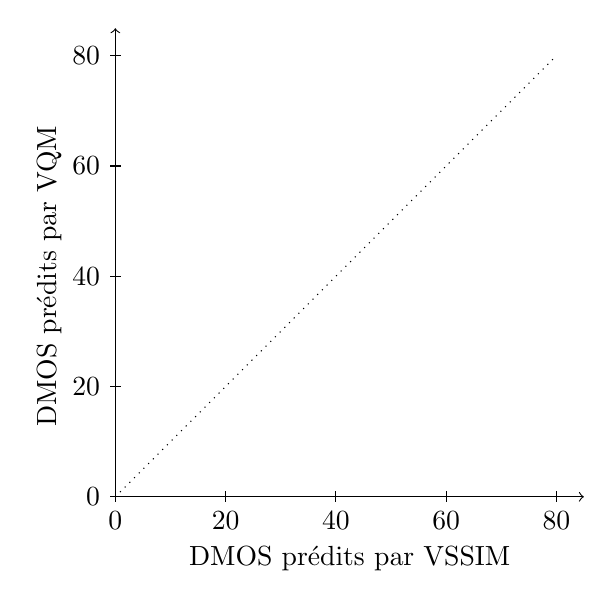
\begin{tikzpicture}[only marks, scale=0.07]
	\pgfsetplotmarksize{1cm}
	\draw plot[mark=+] file {plot/chap5/DMOSpVSSIM-DMOSpVQM-LCD.txt};
	\draw[->] (0,0) -- coordinate (x axis) (85,0);
	\draw[->] (0,0) -- coordinate (y axis) (0,85);
	\foreach \x in {0,20,40,60,80} \draw (\x cm,1cm) -- (\x cm,-1cm) node[anchor=north] {\x};
	\foreach \y in {0,20,40,60,80} \draw (1cm,\y cm) -- (-1cm,\y cm) node[anchor=east] {\y};
	\node[below=0.5cm] at (x axis) {DMOS prédits par VSSIM};
	\node[rotate=90] at (-12,40) {DMOS prédits par VQM};
	\draw[dotted] (0,0) -- (80,80);
\end{tikzpicture}}\hfill
	\subfloat[\label{fig:nuageVQMVSSIMCRT} Mesures sur écran CRT.]{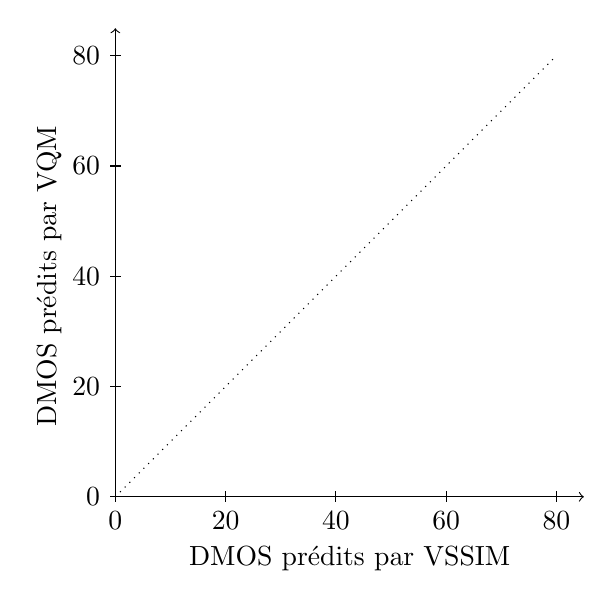
\begin{tikzpicture}[only marks, scale=0.07]
	\pgfsetplotmarksize{1cm}
	\draw plot[mark=+] file {plot/chap5/DMOSpVSSIM-DMOSpVQM-CRT.txt};
	\draw[->] (0,0) -- coordinate (x axis) (85,0);
	\draw[->] (0,0) -- coordinate (y axis) (0,85);
	\foreach \x in {0,20,40,60,80} \draw (\x cm,1cm) -- (\x cm,-1cm) node[anchor=north] {\x};
	\foreach \y in {0,20,40,60,80} \draw (1cm,\y cm) -- (-1cm,\y cm) node[anchor=east] {\y};
	\node[below=0.5cm] at (x axis) {DMOS prédits par VSSIM};
	\node[rotate=90] at (-12,40) {DMOS prédits par VQM};
	\draw[dotted] (0,0) -- (80,80);
\end{tikzpicture}
}\\
  \caption{DMOS prédits par le critère VQM en fonction des DMOS prédits par le critère VSSIM.}
\end{figure}


\section{Conclusion}
Dans un premier temps, ce chapitre a permis de présenter des outils de mesure des performances d'un critère de qualité. Ces outils évaluent les capacités d'un critère à prédire le jugement subjectif. Certains d'entre eux indiquent si deux mesures sont significativement différentes, ce qui permet de comparer différents critères entre eux. Leur intérêt est indiscutable quand à l'analyse des résultats fournis par un critère, alors qu'ils sont rarement utilisés de manière complète dans la littérature.

Dans une seconde phase, nous avons utilisé ces outils pour évaluer les performances de deux critères de qualité vidéo sur la base de séquences haute définition présentée à l'annexe~\ref{annex:base}. Le premier critère évalué est adapté à la vidéo à partir du critère de qualité d'image SSIM~\cite{wang-vqasdm}. Assez simple, celui-ci n'obtient pas de bonnes performances sur la base, avec un coefficient de corrélation maximal de 0,7900 avec les DMOS subjectifs. Le second critère évalué est le modèle \emph{Television} du VQM~\cite{wolf-vqmtech}. Plus performant sur tous les indicateurs, il obtient jusqu'à 0,8981 de coefficient de corrélation linéaire.

Cette étude a permis de dégager trois conclusions majeures :
\begin{itemize}
\item les performances ne sont pas significativement différentes selon que les MOS aient été obtenus avec un écran LCD ou un écran CRT ;
\item la différence de performances dans la prédiction de la qualité visuelle entre les formats TVSD et TVHD est sensible, la qualité de la TVHD étant globalement moins bien prédite ;
\item le critère VQM obtient des coefficients de corrélation et des racines carrées de l'erreur quadratique moyenne significativement meilleurs que VSSIM dans toutes les configurations testées.
\end{itemize}

Ce type d'évaluation, peu courante, montre que les critères conçus pour la télévision standard ne fonctionnent pas aussi bien pour la télévision haute définition. C'est pourquoi il nous a paru nécessaire de proposer des critères adaptés à ce contexte. %C'est l'objet des chapitres suivants.


\ornementChapitre
